\chapter{量子光通信的理论基础}

\section{电磁场的量子态描述}
\subsection{相干态}
通信中常用相干光来传递信息,在数学上,它可以用一个正弦波来表示。
在物理实现上,它可以用线偏振的电场来实现\cite{djordjevic2010fundamentals},
\begin{equation}
\bm{E}(t) = \bm{p} A e^{j\omega t + \phi}.
\end{equation}
上式中,符号$\bm{p}$、$A$、$\omega$和$\phi$分别对应偏振矢量、幅度、频率和相位。
要传递的信息被调制在场的这四个要素上面。
在本文中,主要关注的是对幅度和相位的调制。
这两个要素可以用一个复振幅来描述
\begin{equation}
\alpha = A e^{j\phi}.
\end{equation}
该复振幅也可以用相空间复平面中的一个点来表示,这种相空间图像被称作星座图。
图\ref{fig:signals}展示了OOK、BPSK、QPSK、16-QAM四种常见的调制信号的星座图。

\begin{figure}
\centering
  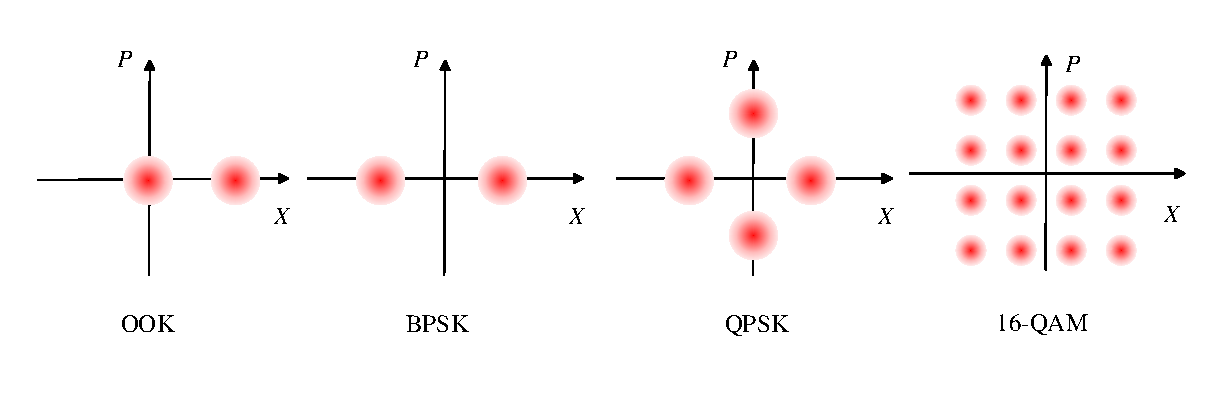
\includegraphics[width=\textwidth]{figures/chap2/signals}
  \caption{常见的四种调制信号星座图}
  \label{fig:signals}
\end{figure}

在量子力学中,电磁场被量子化为若干个不同模式、不同频率的光子\cite{gerry2005introductory,helstrom1976quantum,mandel1995optical}。
单模电磁场的哈密顿量可以表示为无穷个Fork态的线性叠加
\begin{equation}
\hat{H} = \hbar \omega (\hat{a}^\dagger \hat{a} + \frac{1}{2}).
\end{equation}
其中$\hat{a}^\dagger$和 $\hat{a}$ 分别是产生算符和湮灭算符,
乘积$\hat{a}^\dagger \hat{a}$是粒子数算符,他的本振态是Fork态$\ket{n}$,满足
\begin{equation}
\hat{a}^\dagger \hat{a} \ket{n} = n \ket{n}.
\end{equation}

通信中常用的单模相干光脉冲可以用单模相干态$\ket{\alpha}$来描述,它是湮灭算符的本振态
\begin{equation}
\hat{a} \ket{\alpha} = \alpha \ket{\alpha}.
\end{equation}
在Fork态表象中,相干态可以表达为
\begin{equation}
\ket{\alpha} = \exp(-\frac{1}{2}|\alpha|^2) \sum_{n=0}^\infty \frac{\alpha^n}{\sqrt{n!}} \ket{n}.
\end{equation}
如果用光子计数器进行探测,相干态$\ket{\alpha}$探测到的光子数不是一个固定的值,
而是服从泊松分布
\begin{equation}
P_n = |\bra{n}\ket{\alpha}|^2 = \exp(-|\alpha|^2) \frac{|\alpha|^{2n}}{n!} .
\end{equation}
它的平均光子数由
\begin{equation}
\bar{n} = |\alpha|^2
\end{equation}
给出。相干态参数${\alpha}$可以是任何复数,具有复振幅的意义\cite{glauber1963coherent}。

任意两个相干态互不正交,两个相干态的内积为
\begin{equation}
\begin{split}
\bra{\alpha}\ket{\beta} &= \exp(-\frac{1}{2}|\alpha|^2 - \frac{1}{2} |\beta|^2) \sum_{n=0}^\infty \frac{(\alpha^*\beta)^n}{n!} \\
                         &= \exp(\alpha^*\beta -\frac{1}{2}|\alpha|^2 - \frac{1}{2} |\beta|^2).
\end{split}
\end{equation}
恒大于0。相干态互不正交是使得相干态无法完美区分的关键原因。

数学上也常常用密度矩阵来表示信号\cite{wt2001qm},相干态$\ket{\alpha}$也可以用密度矩阵表示为
$\hat{\rho} = \ket{\alpha}\bra{\alpha}$。



\subsection{位移操作}

\begin{figure}
\centering
  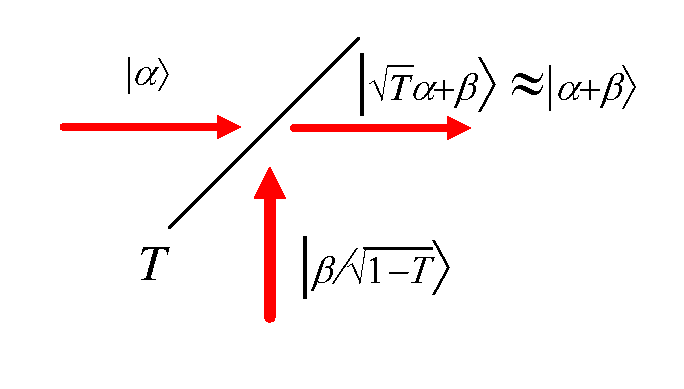
\includegraphics[height=5cm]{figures/chap2/displacement-operator}
  \caption{用波束分束器实现位移操作示意图}
  \label{fig:diaplacement}
\end{figure}

相干态可以通过位移操作进行变换,位移算符定义为\cite{glauber1963coherent,gerry2005introductory,helstrom1976quantum,mandel1995optical}
\begin{equation}
\hat{D}(\alpha) = \exp(\alpha \hat{a}^\dagger - \alpha^* \hat{a}).
\end{equation}
利用位移算符,相干态可以通过对真空态$\ket{0}$位移得到
\begin{equation}
\ket{\alpha} = \hat{D}(\alpha) \ket{0}.
\end{equation}
两个相干态之间也可以通过位移操作进行变换
\begin{equation}
\hat{D}(\beta) \ket{\alpha} = \ket{\alpha + \beta} .
\end{equation}


在实验当中,常用一个相位稳定干涉仪或者波束分束器来实现对相干态的位移操作\cite{cook2007optical,becerra2013experimental,lau2006binary,paris1996displacement}。
图\ref{fig:diaplacement}显示的是利用一个高透过率的波束分束器,
将两个入射场混合输出,近似实现了对其中一个入射场的位移操作,
这种方案在量子接收机实验中经常见到。

\section{经典光通信的接收方案}

在经典光通信中,有三类常见的接收方案,他们分别是
直接检测、零差接收和外差接收。
这三种接收方案受散粒噪声的制约,
使得每一种接收方案存在一个经典极限
——标准量子极限(Standard Quantum Limit)。
接下来,我们简单介绍一下每一种接收方案的具体实现方案。

\subsection{直接检测}



\begin{figure}
\centering
  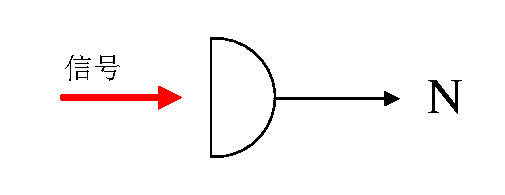
\includegraphics[scale=1]{figures/chap2/DD.pdf}
  \caption{直接检测示意图}
  \label{fig:DD}
\end{figure}


在所有的调制方案中,有一类采用脉冲的有无对信息进行编码,
比如开关键控(OOK)和脉冲位置调制(PPM)。
OOK调制将符号0编码为没有光脉冲,
而将符号1编码为有脉冲;PPM调制则将信息编码到脉冲所在的位置上。
对于这样一类的调制方案,经典光通信中常采用直接检测方案进行探测。
如图\ref{fig:DD}所示,直接检测方案直接探测信号光的强度,
来判断是否存在光脉冲或者光脉冲的幅度\cite{gagliardi1976optical,gagliardi1998optical}。
这种方案可以利用一个光电探测器或单光子探测器实现。
探测器可以输出探测到的光子数目,理想情况下,
对于给定的相干态,探测到$n$个光子的概率
\begin{equation}
\Pr(N = n| \ket{\alpha}) = \frac{|\alpha|^{2n}}{n!} e^{-|\alpha|^2}
\label{eq:dd-prob}
\end{equation}
一般地,对于信号矢态为$\ket{\phi}$的情况下,检测概率为
\begin{equation}
\Pr(N = n| \ket{\phi}) = |\bra{n}\ket{\phi}|^2
\end{equation}



\subsection{零差接收}
零差接收机是一种相干检测方案,如图\ref{fig:HD}所示,
是一种平衡零差接收方案\cite{gagliardi1976optical,gagliardi1998optical}。
这种接收方案和直接检测不同的是,
需要一个本振。对于零差接收本振频率和信号频率一致。
通常本振强度$a_{LO}$远大于信号强度$a_S$,
两路信号通过一个50:50的分束器,
在两个输出口得到两路新的信号$a_+$和$a_-$,满足关系式
\begin{equation}
a_\pm = \frac{a_S \pm a_{LO}}{\sqrt{2}}.
\end{equation}
这两路信号被光电探测器接收,得到两路光电流$i_\pm$。
这两路电流通过一个放大系数为$1/K=1/2q\sqrt{N_{LO}}$的差分放大器,
最后通过一个低通滤波器积分得到输出统计量
\begin{equation}
\alpha_\theta = \frac{N_+ - N_-}{2\sqrt{N_{LO}}}.
\end{equation}
这里假定所有的器件都是理想的。当$N_{LO} \rightarrow \infty$时,
输出统计量服从高斯分布
\begin{equation}
\alpha_\theta \sim N(\Re(ae^{-j\theta}), \frac{1}{4}).
\label{eq:HD-alpha}
\end{equation}
其中$\theta$是本振与信号的相位差。
这种测量方案,用量子力学算符可以用湮灭算符描述为\cite{yuen1980optical,mandel1995optical}
\begin{equation}
\hat{\alpha}_\theta = \Re(\hat{a}_S e^{-j\theta}).
\end{equation}


\begin{figure}
\centering
  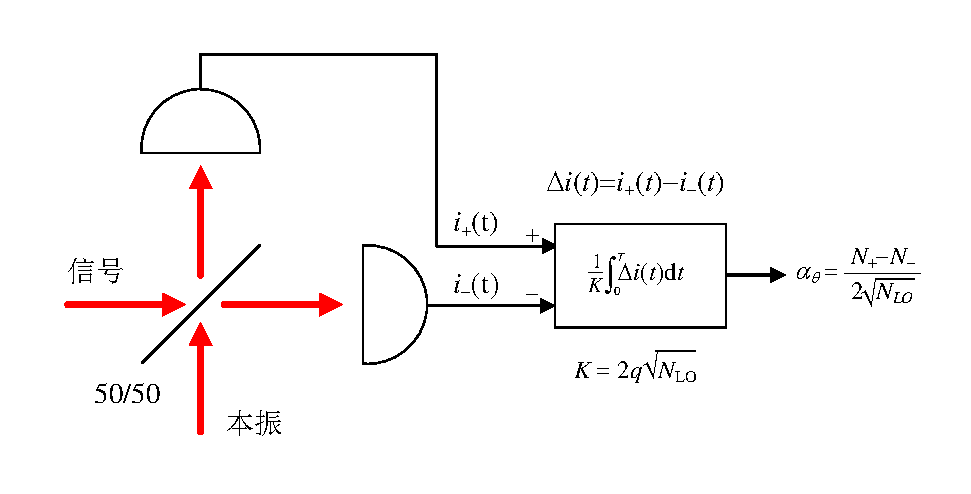
\includegraphics[width=0.8\textwidth]{figures/chap2/homodyne-receiver.pdf}
  \caption{平衡零差检测示意图}
  \label{fig:HD}
\end{figure}

\subsection{外差接收}
在上一小节,我们已经介绍了零差接收方案。
另外一种相干接收方案是外差接收\cite{gagliardi1976optical,gagliardi1998optical},
它采用了与信号频率不同的本振。
图\ref{fig:HeD}是一种平衡外差接收机示意图,
在这种外差接收机中,频率为$\omega$的信号场$a_S$
与频率为$\omega - \omega_{IF}$的强本振场$a_{LO}$
通过一个50:50的分束器混合。
混合后经过光电探测器,得到两路以中频$\omega_{IF}$震荡的电流$i_\pm$。
这两路电流经过一个放大系数为$1/K'=1/q\sqrt{N_{LO}}$的差分放大器,
最后解调出两个正交幅度$\alpha_1$和$\alpha_2$。
假定所有的器件都是理想的,当$N_{LO} \rightarrow \infty$时,
这两个统计量统计独立,分别服从高斯分布
\begin{equation}
\alpha_i \sim N(a_{S_i}, \frac{1}{2}).
\label{eq:Her-receiver-output}
\end{equation}
其中$a_{S_1}=\Re(a_S)$和$a_{S_2}=\Im(a_S)$分别是信号场的两个正交幅度。
这种测量方案,同时测量信号的两个正交幅度,
用量子力学算符湮灭算符可以描述为\cite{yuen1980optical,mandel1995optical}
\begin{equation}
\hat{\alpha}_1 + j \hat{\alpha}_2 = \hat{a}_S.
\label{eq:Her-receiver-output-2}
\end{equation}



\begin{figure}
\centering
  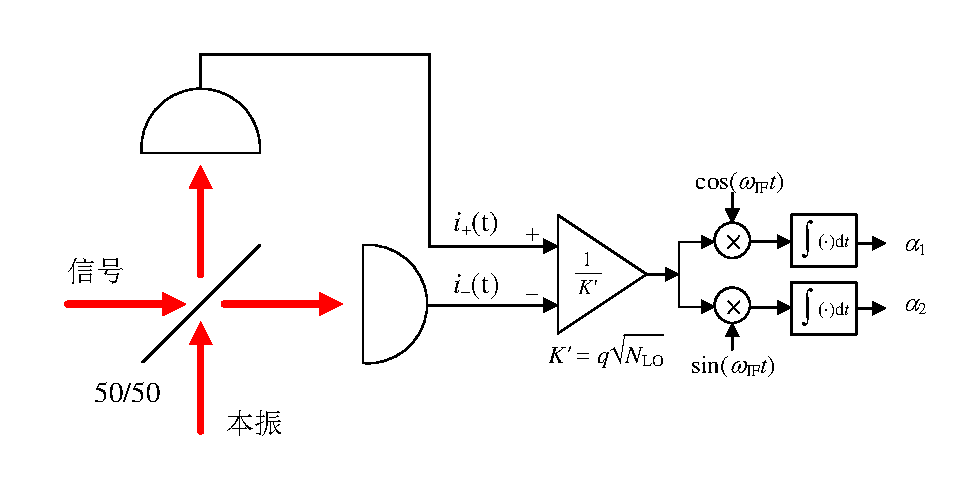
\includegraphics[width=0.8\textwidth]{figures/chap2/heretrodyne-receiver.pdf}
  \caption{平衡外差检测示意图}
  \label{fig:HeD}
\end{figure}


\section{量子检测与估计理论}
\subsection{经典最优检测}
通信系统通常由发送端、信道和接收端三个部分组成。
对某种特定的通信方案,发送端从$M$个符号中以先验概率分布$\zeta_j(j=1,2,...,M)$选择一个发送出去。
先验概率满足归一化条件
\begin{equation}
\sum_{j=1}^M \zeta_j = 1.
\end{equation}
我们称一个假设$H_j (j=1,2,...,M)$是指发送的是第$j$个符号。



在通信的接收端,接收机对电磁场进行探测,可以得到一些统计量。
例如在前面介绍的三种经典监测方案中,输出的统计量分别是光子数目、
$\alpha_\theta$、$\{\alpha_1, \alpha_2\}$。
由于量子涨落和噪声的影响,对于给定的发送信号,
这些统计量通常不是一个固定的值,而是一个随机变量。
一般的,我们假设输出统计量是一个实随机向量$\bm{v} = (v_1, v_2, ..., v_n)$。
当发送第$j$个符号时,
假定它的联合分布为
$p_j(\bm{v}) = p_j(v_1, v_2, ..., v_n)$。
在通信的接收端,通过对接收到的统计量进行判决,
判定发送的符号是哪一个。
下面介绍两种重要的准则——贝叶斯准则和最小错误概率准则。

我们定义决策代价$C_{ij}$为,
当假设$H_j$是正确的情况下,选择了假设$H_i$所需要的代价。
我们期望一个决策是最优的是指该决策所需要的平均代价最小。

我们再来将决策数学化\cite{yzf2002tjxhcl,helstrom1976quantum},
定义在观测到的统计量为$\bm{v}$时,
选择了假设$H_i$的概率为$\pi_i(\bm{v})$,$i=1,2,...,M$。
这些决策概率需满足条件
\begin{equation}
0 \le \pi_i(\bm{v}) \le 1,  \sum_{i=1}^M \pi_i(\bm{v}) = 1.
\label{eq:pi-cond}
\end{equation}
一个简单的例子是一种被称为随机策略的决策方案,
对于任意观测量,这种策略都是随机选择一个假设,
即$\pi_i(\bm{v}) \equiv 1/M, \forall i, \bm{v}$。

在上述符号的约定下,我们可以得到在假设$H_j$是正确的情况下,
策略选择了假设$H_i$的条件概率为
\begin{equation}
\Pr\{i|j\} = \int_{\mathbb{R}^n} \pi_i(\bm{v}) p_j(\bm{v}) d^n \bm{v}.
\end{equation}
这里$\mathbb{R}$代表实数集合,$\mathbb{R}^n$代表$n$维实欧几里得空间。
那么,对所有的观测结果,平均代价为
\begin{equation}
\begin{split}
\bar{C} &= \sum_{i=1}^M \sum_{j=1}^M \zeta_j C_{ij} \Pr{i|j} \\
 &= \sum_{i=1}^M \sum_{j=1}^M \zeta_j C_{ij} \int_{\mathbb{R}^n} \pi_i(\bm{v}) p_j(\bm{v}) d^n \bm{v}.
\end{split}
\end{equation}
对于每一个假设$H_i$,我们定义它的风险函数
\begin{equation}
W_i(\bm{v}) = \sum_{j=1}^M \zeta_j C_{ij} p_j(\bm{v})。
\end{equation}
那么决策的平均代价可以改写为
\begin{equation}
\bar{C} =  \int_{\mathbb{R}^n} \sum_{i=1}^M W_i(\bm{v}) \pi_i(\bm{v}) d^n \bm{v}.
\label{eq:avg-C}
\end{equation}

在式\ref{eq:pi-cond}条件下,最小化式\ref{eq:avg-C},
这是一个凸优化问题。
这个问题可以通过一个简单的观察得以解决。
从式\ref{eq:pi-cond}和\ref{eq:avg-C}可以看出,
对于每一个观测结果$\bm{v} \in \mathbb{R}^n $,要使得平均代价最小,
需要选择风险$W_i(\bm{v})$最小的那一个假设。
即对于每一个观测结果$\bm{v} \in \mathbb{R}^n $,若
\begin{equation}
W_j(\bm{v}) < W_i(\bm{v}), \forall i \neq j,
\end{equation}
那么
\begin{equation}
\pi_j(\bm{v})=1, \pi_i(\bm{v}) \equiv 0, \forall i \neq j.
\end{equation}

为方便记函数
\begin{equation}
\Upsilon(\bm{v}) = \min_j W_j(\bm{v}), 
\end{equation}
那么对所有的观测结果$\bm{v}$和所有的假设$H_i$,有下式成立
\begin{equation}
\begin{split}
[W_i(\bm{v}) - \Upsilon(\bm{v})] \pi_i(\bm{v}) &= 0,  \\
W_i(\bm{v}) - \Upsilon(\bm{v}) &\ge 0.
\label{eq:classic-opt-cond}
\end{split}
\end{equation}
对式\ref{eq:classic-opt-cond}的第一个式子求和,可以得到
\begin{equation}
\Upsilon(\bm{v}) = \sum_i^M W_i(\bm{v})\pi_i(\bm{v}), 
\end{equation}
因此,可以得到最小平均代价为
\begin{equation}
\bar{C}_{min} = \int_{\mathbb{R}^n} \Upsilon(\bm{v}) d^n \bm{v}. 
\end{equation}
容易验证,这样得到的平均代价确实是最小平均代价,
即对任意其他的决策函数$\{\pi_i'(\bm{v})\}$,有
\begin{equation}
\bar{C}' - \bar{C}_{min} = \sum_{i=1}^M \int_{\mathbb{R}^n} [W_i(\bm{v}) - \Upsilon] \pi_i'(\bm{v}) d^n \bm{v} \ge 0. 
\end{equation}


现代的文献中,常将这种最小化平均代价函数的决策称作贝叶斯准则。
在这当中,有一种被称为最小错误概率准则的策略,它的决策代价系数定义为
\begin{equation}
C_{ii} = -1; C_{ij}=0, \forall i\neq j. 
\label{eq:min-err-cond}
\end{equation}
在这种决策代价下,最小平均代价就是最小平均错误概率
\begin{equation}
P_e = 1 - \sum_{j=1}^M \zeta_j \Pr{j|j} = \sum_{j=1}^M \zeta_j \sum_{k\neq j}\Pr{k|j}.
\end{equation}
在通信中,常用最小平均错误概率准则来设计接收机的接收策略。
因此本文也主要以该准则来设计量子接收机。

通过经典的三种探测方式加上经典检测预估计理论所得到的最佳接收方案,
它能达到的最小平均错误概率通常被称作标准量子极限(SQL)。




\subsection{量子最优检测}
上世纪六十年代,C.W. Helstrom和H. P. Yuen等人
将假设检验理论与量子力学结合起来,
发展出一套适用于量子测量的量子检测与估计理论
\cite{helstrom1976quantum,helstrom1967detection,yuen1975optimum}。
根据这一套理论,可以从理论上给出最优检测的数学形式,
下面我们简单回顾一下这个理论的主要内容。

在量子力学中,一个测量在数学上被描述为一个正定算子值测量(POVM)算符\cite{helstrom1976quantum}。
如果用算符$\hat{\Pi}_i (i=1,2,...,M)$表示一组POVM测量,
那么一组完备的POVM测量需要满足条件
\begin{equation}
\begin{split}
\hat{\Pi}_i & \ge 0, \\
\sum_{i=1}^M \hat{\Pi}_i & = \hat{I}.
\end{split}
\end{equation}

例如,直接检测利用POVM算符可以表达为
\begin{equation}
\hat{\Pi}_n = \ket{n}\bra{n}, n=0,1,2,...
\end{equation}
其中$\ket{n}$是Fork态矢量,这是一组正交投影测量。
我们说一组测量是正交投影测量是指它们满足正交条件
\begin{equation}
\hat{\Pi}_i \hat{\Pi}_j = 0, \forall i \neq j
\end{equation}
和投影算符条件
\begin{equation}
\hat{\Pi}_n^2 = \hat{\Pi}_n, n=0,1,2,...
\end{equation}
如果直接检测采用ON-OFF探测器,即只能探测到有光子还是没有光子,
那么直接检测对应于一个二元测量
\begin{equation}
\hat{\Pi}_0 = \ket{0}\bra{0}, \hat{\Pi}_1 = \hat{I} - \ket{0}\bra{0}.
\end{equation}


假设发送的信号态用密度矩阵为$\hat{\rho}_j$,那么将符号$j$检测为符号$i$的条件概率为
\begin{equation}
\Pr(i|j) = \Tr(\hat{\rho}_j \hat{\Pi}_i), (i,j)=1,2,...,M.
\end{equation}
那么利用上一节的符号定义,在这样的信号和测量设置下,
总的平均代价为
\begin{equation}
\bar{C} =  \sum_{i=1}^M \sum_{j=1}^M \zeta_jC_{ij} \Tr(\hat{\rho}_j \hat{\Pi}_i) \\
        =  \Tr \sum_{i=1}^M \hat{W}_i \hat{\Pi}_i.
\label{eq:q-avg-C}
\end{equation}
这里,风险算符$\hat{W}_i$定义为
\begin{equation}
\hat{W}_i = \sum_{j=1}^M \zeta_jC_{ij}\hat{\rho}_j.
\end{equation}
这样,我们得到与经典检测理论对应的优化问题。
H. P. Yuen和C. W. Helstrom等人给出该优化问题的一个充要条件,
\begin{equation}
\begin{split}
(\hat{W}_i - \hat{\Upsilon})\hat{\Pi}_i = \hat{\Pi}_i(\hat{W}_i - \hat{\Upsilon}) & = \bm{0}, i=1,2,...,M,  \\
\hat{W}_i - \hat{\Upsilon} & \ge \bm{0}, i=1,2,...,M.
\label{eq:optim-povm-cond}
\end{split}
\end{equation}
其中拉格朗日算符
\begin{equation}
\hat{\Upsilon} = \sum_{j=1}^M \hat{\Pi}_j\hat{W}_j = \sum_{j=1}^M\hat{W}_j\hat{\Pi}_j.
\end{equation}
那么,最小平均代价可以简化为
\begin{equation}
\bar{C}_{min} = \Tr(\hat{\Upsilon}).
\end{equation}

若取式\ref{eq:min-err-cond}中的最小平均错误概率准则决策代价系数,
那么最优检测问题可以简化为
\begin{equation}
\begin{split}
\max_{\hat{\Pi}_i}  \quad  &  \sum_{i=1}^M \Tr(\hat{\rho}_i'\hat{\Pi}_i) \\
s.t. \quad  & \hat{\Pi}_i \ge 0, i=1,2,...,M   \\
     \quad  & \sum_{i=1}^M \hat{\Pi}_i = \hat{I}.
\end{split}
\end{equation}
上式中,$\hat{\rho}_i' = \zeta_i \hat{\rho}_i$。
该问题是一个半正定规划(SDP)问题,
需要求解的未知矩阵个数是$M$,
可以通过求解其对偶问题将问题简化
为未知矩阵只有1个的半正定规划问题\cite{eldar2003designing}
\begin{equation}
\begin{split}
\min_{\hat{X}}  \quad & \Tr(\hat{X}) \\
s.t.          \quad & \hat{X} \ge \hat{\rho}_i', i=1,2,...,M.
\label{eq:Hel-SDP}
\end{split}
\end{equation}
利用一种为Matlab编写的凸优化工具箱CVX,
可以很方便地求解上述半正定规划问题\cite{cvx,gb08}。

利用量子检测预估计理论计算出来的最小错误概率,
通常称作这种信号的Helstrom极限,
通常比经典检测方案所能达到的极限要低很多\cite{helstrom1976quantum}。



\subsection{平方根检测}
一般情况下,为了求解量子最优测量问题,
需要利用数值优化工具进行数值计算,
只有很少数情况下可以得到解析表达式。
因此,这不利于理论研究。
而平方根检测是一种解析方法,它利用通过信号矢量的Gram矩阵的平方根
构造出来的一组POVM算符进行测量\cite{hausladen1994pretty,hausladen1996classical}。
在最小错率概率准则下,它是一种近最优的检测方案,
但是在最小均方误差准则下,它是最优测量。
并且,在信号具有几何均匀对称性的情况下,
它也是最小错误概率准则下的最优检测\cite{kato1999quantum,eldar2001quantum,cariolaro2010performance,cariolaro2010theory}。
在很多理论问题的研究中,由于平方根检测具有良好的解析表达式,
常常被用来作为一种理论检测方案进行研究\cite{hausladen1996classical,sasaki1998quantum,guha2012polar}。
下面,我们介绍一下这种接收方案的数学形式。

设$M$个信号由$n$维Hilbert空间$\mathcal{H}$中
的向量表示为$\ket{\psi_i}(i=1,2,...M)$,对应的密度矩阵为
$\hat{\rho}_i = \ket{\psi_i} \bra{\psi_i}$。
这些信号张成$\mathcal{H}$中一个$r\le M$维子空间$\mathcal{U}$。
当且仅当$M$个信号线性独立时,等号成立$r=M$。
$M$个POVM测量满足
\begin{equation}
\hat{\Pi}_i \ge 0, \sum_{i=1}^M \hat{\Pi}_i = \hat{I}_r.
\end{equation}
这里$\hat{I}_r$是子空间$\mathcal{U}$上的单位矩阵。

将信号的密度矩阵和POVM测量矩阵分解为
\begin{equation}
\begin{split}
\hat{\rho}_i & = \hat{\gamma}_i \hat{\gamma}_i^\dagger,\\
\hat{\Pi}_i & = \hat{\mu}_i \hat{\mu}_i^\dagger.
\end{split}
\end{equation}
重新定义信号集合矩阵$\hat{\Gamma}=[\hat{\gamma}_1 \quad \hat{\gamma}_2 \quad ...\quad \hat{\gamma}_M]$
和POVM测量集合矩阵$\hat{M} = [\hat{\mu}_1\quad \hat{\mu}_2\quad ...\quad \hat{\mu}_M]$。
Gram矩阵定义为$\hat{T} = \hat{\Gamma} \hat{\Gamma}^\dagger$
和$\hat{G} = \hat{\Gamma}^\dagger \hat{\Gamma}$,
平方根检测给出的POVM测量集合矩阵为
\begin{equation}
\hat{M} = \hat{T}^{-\frac{1}{2}} \hat{\Gamma} = \hat{\Gamma} \hat{G}^{-\frac{1}{2}}.
\end{equation}
可以证明这种POVM测量使得均方误差
\begin{equation}
E = \Tr[(\hat{\Gamma} - \hat{M})^\dagger (\hat{\Gamma} - \hat{M})]
\end{equation}
达到最小值\cite{eldar2001quantum}。

在平方根检测的POVM测量算符下,
将信号$i$判断为$j$的条件概率为
\begin{equation}
\begin{split}
\Pr{j|i} = \Tr(\hat{\rho}_i \hat{\Pi}_j) & = \Tr(\hat{\gamma}_i \hat{\gamma}_i^\dagger \hat{\mu}_j \hat{\mu}_j^\dagger) \\
     =\Tr(\hat{\mu}_j^\dagger\hat{\gamma}_i \hat{\gamma}_i^\dagger \hat{\mu}_j )     & = \Tr(\hat{B}_{ji} \hat{B}_{ji}^\dagger).
\end{split}
\end{equation}
这里矩阵$\hat{B}_{ji}$是矩阵 $\hat{M}^\dagger \hat{\Gamma} = \hat{G}^{1/2}$的第$(j,i)$子块$\hat{\mu}_j^\dagger\hat{\gamma}_i$。
对于纯态信号集合,信号密度矩阵秩为1,因此$\hat{\gamma}_i$和$\hat{\mu}_i$是一个向量,
因此
\begin{equation}
\Pr{j|i} = |(\hat{G}^{1/2})_{ji}|^2.
\end{equation}
所以,若先验概率相同的情况下,平均错误概率为
\begin{equation}
P_e = 1 - \frac{1}{M}\sum_{i=1}^M |(\hat{G}^{1/2})_{ii}|^2.
\label{eq:SRM-Pe}
\end{equation}


如果信号满足几何均匀对称性,即存在幺正矩阵$\hat{U}$使得
\begin{equation}
\hat{\rho}_i = \hat{U}^{i-1} \hat{\rho}_1 \hat{U^\dagger} ^ {i-1}
\end{equation}
成立。那么,可以验证平方根检测满足最优检测的充要条件\cite{eldar2001quantum},
即公式\ref{eq:optim-povm-cond}成立。
并且,此时Gram矩阵$\hat{G}$是循环矩阵,
设$\lambda_i(i=1,2,...,M)$是其$M$个特征值,
那么式\ref{eq:SRM-Pe}可以进一步简化为\cite{kato1999quantum}
\begin{equation}
P_e = 1 - \frac{1}{M^2} (\sum_{i=1}^M \sqrt{\lambda_i})^2.
\label{eq:SRM-Pe-GUS}
\end{equation}

容易验证M阶PSK信号密度矩阵可以通过幺正矩阵\cite{kato1999quantum}
\begin{equation}
\hat{U} = \exp(j\frac{2\pi}{M} \hat{n})
\end{equation}
相似。其中$\hat{n}=\hat{a}^\dagger \hat{a}$是粒子数算符。
对于M阶PPM,对应的幺正矩阵是一个排列矩阵\cite{cariolaro2010theory}
\begin{equation}
\hat{U} = \sum_{k=1}^n \omega_n(k) \otimes \hat{I}_H \otimes \omega_n^*(k).
\end{equation}
其中$\omega_n(k)$是一个$n$维向量,
它的第$k$维为1,其它维都是0。
$\hat{I}_H$是一个$H=n^{M-1}$阶单位矩阵。

因此,对于OOK、M阶PSK、M阶PPM信号,
平方根检测都是最优检测。
对于QAM信号,平方根检测不是最优的测量,但是非常接近最优。
图\ref{fig:SRM-vs-Hel}显示的是16-QAM平方根检测(SRM)和
通过半正定规划计算出来的最优检测性能(Helstrom)差异。
可以看到只在小信号区域有明显差异。

\begin{figure}
\centering
  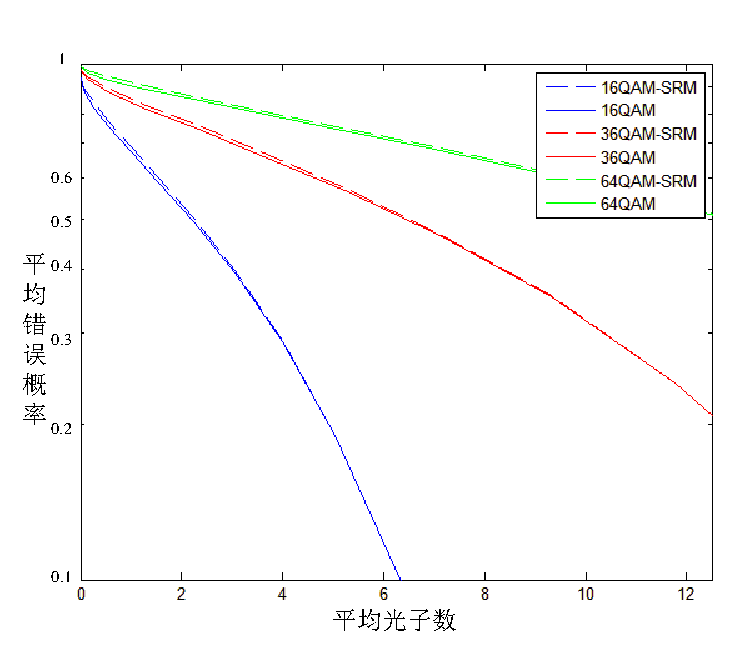
\includegraphics[width=0.6\textwidth]{figures/chap2/QAM-SRM-vs-Helstrom}
  \caption{QAM信号平方根检测(SRM)性能与Helstrom极限}
  \label{fig:SRM-vs-Hel}
\end{figure}


\section{现有的量子接收机简介}
自量子检测与估计理论提出以来,如何用现有的物理器件来实现量子接收机,
成为很多研究者关心的问题。二十世纪七十年代,Kennedy和Dolinar等人
首先对二元调制进行探究,分别提出利用线性光学元件实现的Kennedy接收机
和Dolinar接收机\cite{kennedy1973near,dolinar1973optimum}。
后来,经过后续研究者的进一步探索,更多的接收方案
也被提出来了。在本章中,我们回顾一下已被提出的一些重要的接收机
实现方案。
\subsection{二元调制信号量子接收机}
首先,我们来看一些最简单的调制方案——二元调制。
它包括被广泛应用的两种调制方案——OOK和BPSK。
图\ref{fig:signals}显示了他们在星座图上的图像。



这两种调制的最优量子检测性能被Helstrom给出\cite{helstrom1976quantum},
也可以通过平方根检测得到。因为这种两种调制方案是几何均匀对称的,
其对应的幺正矩阵是位移算符$\hat{D}(\alpha)$和$\hat{D}(2\alpha)$,
所以平方根检测性能就是最优量子检测的性能。
我们先求出对应的Gram矩阵
\begin{equation}
\hat{G} = \begin{bmatrix}
            1  &   \xi  \\
            \xi^*  &  1
          \end{bmatrix}
\label{eq:OOK-BPSK-Gram}
\end{equation}
其中$\xi$是两个符号对应的向量的内积,
对于OOK信号,
\begin{equation}
\xi = \bra{0}\ket{\alpha} = e^{-\frac{1}{2}|\alpha|^2},
\end{equation}
而对BPSK信号,
\begin{equation}
\xi = \bra{-\alpha}\ket{\alpha} = e^{-2|\alpha|^2}.
\end{equation}
利用Gram矩阵的表达式\ref{eq:OOK-BPSK-Gram},容易计算出它
的两个特征值为$\lambda_{1,2} = 1 \pm |\xi|$。
根据式\ref{eq:SRM-Pe-GUS},可得平均错误概率为
\begin{equation}
\begin{split}
P_e  &= 1 - \frac{1}{4}(\sqrt{\lambda_1} + \sqrt{\lambda_2})^2\\
     & = \frac{1}{2} \left(1 - \sqrt{1 - |\xi|^2} \right).
\label{eq:OOK-BPSK-Pe-Hel}
\end{split}
\end{equation}

对于BPSK调制集合$\{\ket{-\alpha}, \ket{\alpha} \}$,
在1973年的时候,Kennedy提出\cite{kennedy1973near}利用一个本振场,
对信号进行位移操作$\hat{D}(\alpha)$,
将信号集合变成OOK调制$\{\ket{0}, \ket{2\alpha} \}$,
然后进行直接探测,如图\ref{fig:kennedy-receiver}所示。
如果没有检测到光子(OFF),就判决为信号$\ket{-\alpha}$,
否则(ON)判决为信号$\ket{\alpha}$。
假设$H_0$代表信号$\ket{-\alpha}$,假设$H_1$代表信号$\ket{\alpha}$。
那么,理想条件下,探测的条件概率为
\begin{equation}
\begin{split}
P(\text{OFF}|H_0) & = 1, \\
P(\text{ON}|H_1)  & = 1 - |\bra{0}\ket{2\alpha}|^2 \\
                  & = 1 - e^{-4|\alpha|^2}.
\end{split}
\end{equation}
在通信系统中,先验概率通常是相同的,为$1/2$,那么这种探测的平均错误概率为
\begin{equation}
P_e  = 1 - P(H_0)P(\text{OFF}|H_0) - P(H_1)P(\text{ON}|H_1) = \frac{1}{2}e^{-4|\alpha|^2}.
\label{eq:BPSK-Kennedy}
\end{equation}


\begin{figure}
\centering
  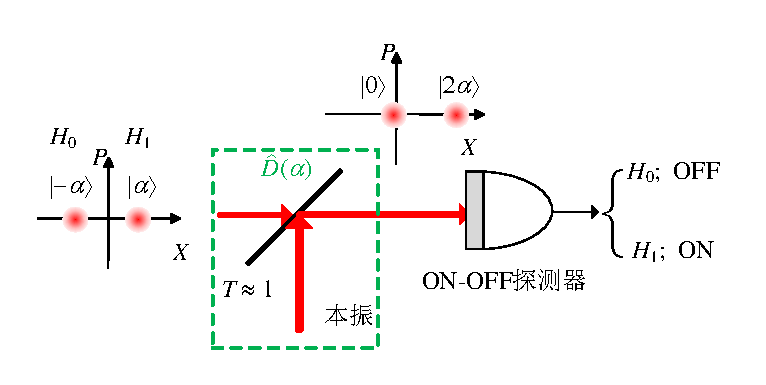
\includegraphics[width=0.8\textwidth]{figures/chap2/Kennedy-receiver}
  \caption{Kennedy接收机示意图}
  \label{fig:kennedy-receiver}
\end{figure}


经典通信系统中,常采用零差接收来探测BPSK信号。
这里假定$\alpha$是实数,根据式\ref{eq:HD-alpha},取$\theta=0$,可知平均错误概率为
\begin{equation}
\begin{split}
P_e & = 1 -\sqrt{\frac{2}{\pi}}\int_0^{\infty} e^{-2(x - \alpha)^2} dx \\
    & = \frac{1}{2}\erfc(\sqrt{2}\alpha).
\end{split}
\end{equation}
对于BPSK信号,经典的零差接收机性能也叫它的标准量子极限(SQL)。
当光子数很大时,利用余误差函数$\erfc$的Chernoff界\cite{chang2011chernoff},
当$x \gg 1$时,$\erfc(x) \approx e^{-x^2}$,
可以得到BPSK零差接收机的渐进性能为
\begin{equation}
P_e = \frac{1}{2}\erfc(\sqrt{2}\alpha) \approx \frac{1}{2} e^{-2\alpha^2}.
\label{eq:BPSK-HD-approx}
\end{equation}
对比式\ref{eq:BPSK-Kennedy}和\ref{eq:BPSK-HD-approx}可以看出,
当光子数较大时,Kennedy接收机的性能比经典的零差接收具有指数倍的增益。
对式\ref{eq:OOK-BPSK-Pe-Hel}做大信号近似,可得在$|\alpha|^2 \gg 1$时,
\begin{equation}
\begin{split}
P_e &= \frac{1}{2} (1 - \sqrt{1 - e^{-4|\alpha|^2}}) \\
    &\approx \frac{1}{4} e^{-4|\alpha|^2}.
\label{eq:BPSK-Hel-approx}
\end{split}
\end{equation}
对比式\ref{eq:BPSK-Kennedy}和\ref{eq:BPSK-Hel-approx}可以看出,
在大信号时,Kennedy接收机与理想的最优量子检测只相差一个常数因子$1/2$,
即Kenendy接收机距最优量子检测只相差3dB。
数值仿真结果如图\ref{fig:Kennedy-error}所示,
可以看到在光子数较小的时候,Kennedy接收机性能没有突破标准量子极限,
只在大信号时能够突破标准量子极限。


\begin{figure}
\centering
  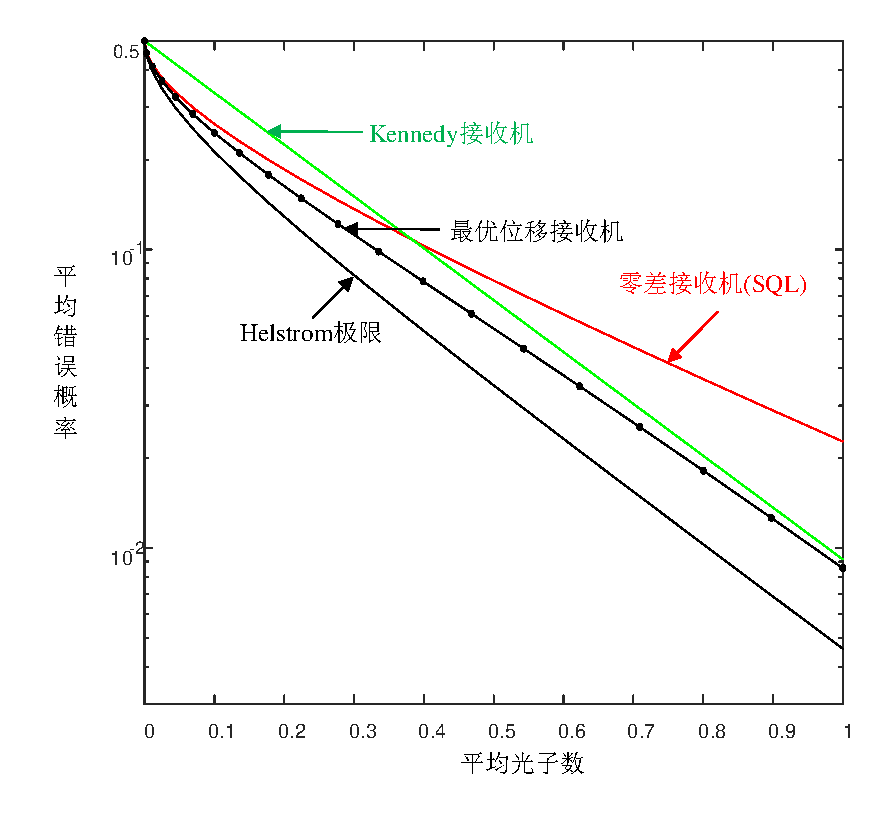
\includegraphics[width=0.6\textwidth]{figures/chap2/Kennedy-error}
  \caption{BPSK信号Kennedy接收机性能曲线}
  \label{fig:Kennedy-error}
\end{figure}


为了解决Kennedy接收机在小信号时的不足,一种采用最优位移
的广义Kennedy接收机(也叫最优位移接收机)被提出\cite{takeoka2008discrimination}。
这种接收机采用与Kennedy接收机相同的结构,但是采用的位移操作
是$\hat{D}(\beta)$,其中位移参数$\beta$通过优化得到。
在这种参数配置下,易得接收机的错误概率为
\begin{equation}
\begin{split}
P_e &= \frac{1}{2} (1 - e^{-|\alpha-\beta|^2} + e^{-|\alpha+\beta|^2}) \\
    &= \frac{1}{2} - e^{-\alpha^2-\beta^2} \sinh(2\alpha\beta).
\label{eq:BPSK-Opt-Kennedy}
\end{split}
\end{equation}
最优位移参数通过求解方程$\partial P_e / \partial \beta  = 0$
得到,即
\begin{equation}
\tanh(2\alpha\beta) = \frac{\alpha}{\beta}.
\end{equation}
从图\ref{fig:Kennedy-error}中可以看到,
最优位移接收机在光子数较小的时候也能突破标准量子极限。
随着光子数增大,最优位移接收机和Kennedy接收机性能越来越接近。
事实上,当光子数很大时,$\tanh(2\alpha\beta) \rightarrow 1$,
最优位移量$\beta \rightarrow  \alpha$。


1973年,Kennedy的学生Dolinar提出Dolinar接收机。
在Kennedy接收机的基础上,Dolinar接收机增加了对本振的实时反馈控制\cite{dolinar1973optimum}。
如图\ref{fig:Dolinar-receiver}所示,位移操作$\hat{D}(\beta)$
的位移量$\beta$在两个策略$u_1(t)$和$u_2(t)$中选择,
每一次单光子探测器接收到一个光子,就切换到另一个位移策略上去。
并且每一个位移策略都是随时间变化的函数。
这里本振的最优控制策略可以通过最优控制理论优化得到\cite{geremia2004distinguishing}。
当本振采用最优控制策略的情况下,可以证明Dolinar接收机
可以达到Helstrom极限,是理论上的最优检测方案\cite{dolinar1973optimum,geremia2004distinguishing}。
2007年,Cook等人从实验上实现了OOK调制的Dolinar接收机\cite{cook2007optical}。

\begin{figure}
\centering
  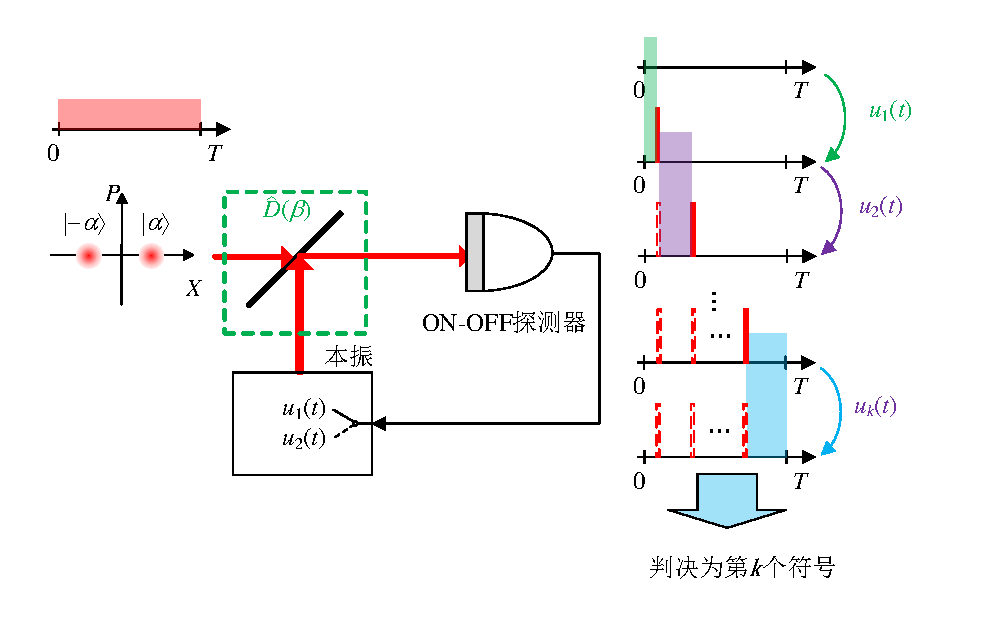
\includegraphics[width=\textwidth]{figures/chap2/Dolinar-receiver}
  \caption{Dolinar接收机原理图}
  \label{fig:Dolinar-receiver}
\end{figure}

Dolinar接收机需要实时反馈控制,这对工程实现要求过高。
一些分区检测方案通过将信号在时间上或者能量上分成
若干份,然后分别采用最优位移接收,弥补了这个不足\cite{vilnrotter2012quantum,li2013optimal,sych2014optimal}。
当分区数目趋近于无穷大时,这种接收机的理论性能和Dolinar接收机一致\cite{sych2014optimal}。

\subsection{多元调制信号量子接收机}
上一小节,我们回顾了最简单的调制信号——二元调制。
这一节我们回顾一下目前研究的比较多的多元调制信号——PSK调制和PPM调制。

QPSK信号用相干态可以表示为
\begin{equation}
\ket{\alpha_i} = \ket{\alpha e^{j \frac{\pi}{2} (i-2)}},i=1,2,3,4.
\end{equation}
我们先来计算一下它的标准量子极限,对于QPSK信号,
外差接收机的性能就是它的标准量子极限。
利用式\ref{eq:Her-receiver-output}或式\ref{eq:Her-receiver-output},
可以得外差接收机平均错误概率为\cite{helstrom1976quantum,kato1999quantum}
\begin{equation}
\begin{split}
P_e &= 1 - \frac{1}{\pi}\int_{Q_1} \exp(-|\beta-\alpha|^2) d^2 \beta \\
    &= 1 - \frac{1}{\pi}\int_0^{\infty} dr \int_{-\pi/4}^{\pi/4} \exp(-\alpha^2 - r^2 + 2\alpha r \cos \theta) r d\theta .
\end{split}
\end{equation}
上式中$Q_1$代表复平面上的区域 $\{\beta|-\pi/4 \le \arg \beta < \pi/4\}$。
%当光子数很大的时候$|\alpha|^2 \gg 1$,利用余误差函数的Chernoff界\cite{chang2011chernoff},
%可得其渐近性能为
%\begin{equation}
%\begin{split}
%P_e &= [2 - \erfc(|\alpha|)]\erfc(|\alpha|) \\
%    &\approx 2e^{-|\alpha|^2}.
%\end{split}
%\end{equation}

因为QPSK具有几何均匀对称性,所以平方根检测就是其最优检测。
QPSK信号对应的Gram矩阵为
\begin{equation}
G = \left[
\begin{array}{cccc}
 1 & e^{-n} & e^{-2 n} & e^{-n} \\
 e^{-n} & 1 & e^{-n} & e^{-2 n} \\
 e^{-2 n} & e^{-n} & 1 & e^{-n} \\
 e^{-n} & e^{-2 n} & e^{-n} & 1 \\
\end{array}
\right].
\end{equation}
这里$n = |\alpha|^2$是信号平均光子数。
根据Gram矩阵可以计算出它的四个特征值为
\begin{equation}
\begin{split}
\lambda_{1,2,3,4} = & e^{-2 n} \left(e^n-1\right)^2,e^{-2 n} \left(e^n+1\right)^2, \\
                    & e^{-2 n} \left(e^{2 n}-1\right),e^{-2 n} \left(e^{2 n}-1\right).
\end{split}
\end{equation}
因此,根据式\ref{eq:SRM-Pe-GUS}可得
\begin{equation}
P_e = 1-\frac{1}{4} \left(\sqrt{1-e^{-2 n}}+1\right)^2.
\label{eq:QPSK-Hel-error}
\end{equation}
在大光子数$n \gg 1$近似条件下,渐近性能为
\begin{equation}
\begin{split}
P_e &= 1-\frac{1}{4} (2 - e^{-2n} + 2\sqrt{1-e^{-2n}}) \\
    &\approx 1-\frac{1}{4} (2 - e^{-2n} + 2- e^{-2n}) \\
    &= \frac{1}{2} e^{-2n} =  \frac{1}{2} e^{-2|\alpha|^2}.
\label{eq:QPSK-Hel-approx}
\end{split}
\end{equation}


\begin{figure}
\centering
  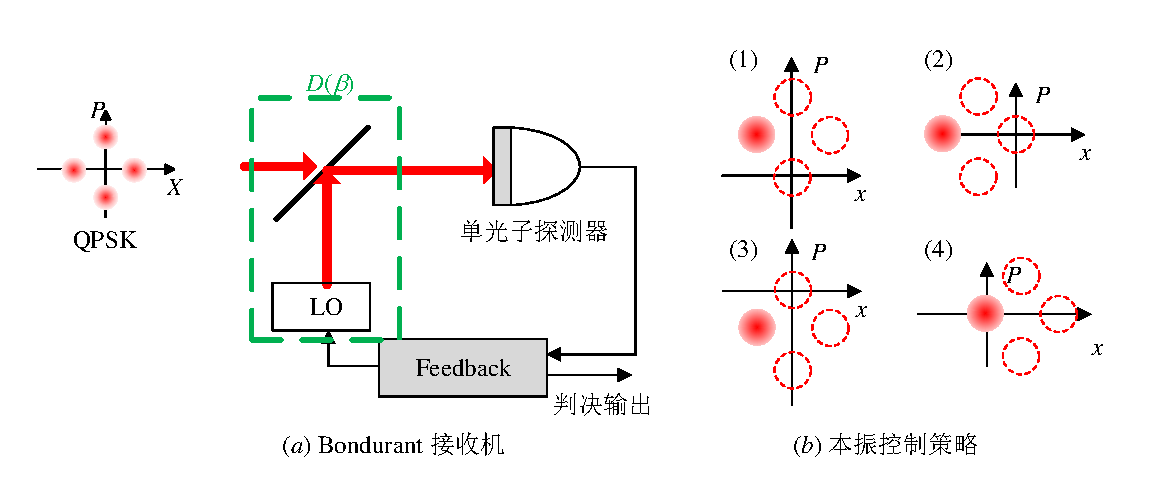
\includegraphics[width=\textwidth]{figures/chap2/QPSK-Bondurant-receiver}
  \caption{QPSK信号Bondurant接收机原理图及反馈控制策略}
  \label{fig:QPSK-Boundurant-receiver}
\end{figure}


1993年,MIT林肯实验室的R. S. Bondurant将Dolinar接收机
的反馈策略推广到QPSK信号,提出两种Bondurant接收机。
这两种接收机只在反馈策略上有所差异,其它都相同\cite{bondurant1993near}。
如图\ref{fig:QPSK-Boundurant-receiver} (\textit{a})所示,
Bondurant接收机由波束分束器、单光子探测器以及一个受反馈控制的本振构成。

第一种Bondurant接收机可以用图\ref{fig:QPSK-Boundurant-receiver} (\textit{b}) 来说明,
在符号开始的时候,接收机选择假设$H_1$,
即假设接收到的符号为$\ket{\alpha_1}$,
反馈策略控制本振将符号1归零,
即控制位移操作$\hat{D}(\beta) = \hat{D}(-\alpha_1)$。
如果在整个符号周期都没有光子计数时间发生,那么选择假设$H_1$输出。
否则,在符号周期中的某个时刻,单光子探测器探测到光子,
那么假设不成立。接着,反馈策略立即控制本振,归零符号2,
即选择假设$H_2$。然后重复上一步,如果继续有光子计数,
则归零符号3,选择假设$H_3$。如果仍然有光子计数,
那么归零符号4,选择假设$H_4$。理想情况下,最多有3个光子计数时间发生。
符号周期结束的时候,选择当前的假设输出。
和Dolinar接收机一样,Bondurant接收机也采用实时反馈控制策略,
但是在每两个光子到达的时间间隔之间,Bondurant接收机的本振是恒定的。

若先验概率相同,第一种Bondurant接收机的平均错误概率为\cite{bondurant1993near}
\begin{equation}
P_e = (\frac{3}{4} + |\alpha|^2) e^{-2|\alpha|^2}.
\end{equation}
当平均光子数较大的时候,渐近性能为
\begin{equation}
P_e \approx |\alpha|^2 e^{-2|\alpha|^2}.
\label{eq:QPSK-Bondurant-approx}
\end{equation}
对比\ref{eq:QPSK-Hel-approx}和\ref{eq:QPSK-Bondurant-approx}
可以看出,第一种Bondurant接收机渐近性能的指数项与最优检测相同。

对于第二种Bondurant接收机,
也是依次归零符号1符号2,但是
在第2个光子到达的时候,反馈控制策略有所不同。
设$t_1$和$t_2$分别代表第1个光子和第2个光子达到的时间。

(a) 如果 $t_1 \le t_2 - t_1$,那么归零符号3,
如果没有光子计数发生了,则选择假设3,否则选择假设4。

(b) 如果 $t_1 > t_2 - t_1$,那么归零符号4,
如果没有光子计数发生了,则选择假设4,否则选择假设3。

在这种策略配置下,接收机的平均错误概率为\cite{bondurant1993near}
\begin{equation}
\begin{split}
P_e  =& \frac{9}{4} e^{-2n} - 2 e^{-3n} + n e^{-3n} \\
      &  + \frac{1}{2} e^{-4n} - n e^{-4n}. 
\end{split}
\end{equation}
上式中$n=|\alpha|^2$为信号平均光子数。
当光子数很大时,略去高阶小量,得到第2中Bondurant接收机渐近性能为
\begin{equation}
P_e \approx \frac{9}{4} e^{-2n} = \frac{9}{4} e^{-2|\alpha|^2}.
\label{eq:QPSK-Bondurant2-approx}
\end{equation}
对比\ref{eq:QPSK-Hel-error}和\ref{eq:QPSK-Bondurant2-approx}两式
可知,第2中Bondurant接收机渐近性能和最优检测只相差一个常数,比第一种
Bondurant接收机前进了一步。

这两种接收机虽然在信号较大的时候可以突破标准量子极限,
但是在小信号的时候,并没有突破标准量子极限。
后来M{\"u}ller借鉴最优位移接收机的思想,
采用不精确归零的方法,改进了小信号时的
性能,使得Bondurant接收机可以在任意光子数都能突破标准量子极限\cite{muller2014qpsk,muller2014m}。

由于Bondurant接收机也需要实时反馈控制,因此不利于工程实现。
后续的研究者 Izumi 通过前馈的方式,将每一个PSK信号分成若干份,
采用Bondurant接收机相似的策略进行前馈\cite{izumi2012displacement}。通过
这种方式减少了反馈带宽的需求,但是同时却增加了
资源的消耗。

后面的研究者Becerra将最大后验概率归零策略加入归零顺序之中,
在每一次前馈的过程中,选择在当前时刻具有最大后验概率的符号,
进行归零\cite{becerra2011m}。这种策略,可以有效地降低
接收机的平均错误概率。2013年,Becerra用反馈的方式
从实验上对这种策略进行了验证\cite{becerra2013experimental}。
并且,考虑到非理想因素如暗计数、模式失配的影响,
将接收端的探测器换成具有光子数分辨能力的探测器,
可以有效的提高接收机的鲁棒性,可以降低暗计数和模式失配带来的
不利影响\cite{izumi2013quantum,li2013suppressing}。
这个结论也在2015年被Becerra通过实验验证\cite{becerra2015photon}。

至此,原则上可以在实验上实现具有鲁棒性的量子接收机,
但是理论上的最优检测如何实现,仍然是一个需要继续研究的问题。

与上述思想不同的是,M{\"u}ller等人提出一种利用
一个零差接收机和一个Kennedy接收机实现QPSK信号接收的
混合接收机\cite{muller2012quadrature}。
这种方案不用反馈控制,简化了QPSK信号接收机的实现。
这种结构也被K. Li推广到16-QAM信号\cite{李科2014}。

在前面我们回顾了PSK信号的量子接收机,
接下来我们回顾一下PPM信号量子接收机研究现状。

首先,我们来计算一下M阶PPM的标准量子极限。
M阶PPM信号有M个时隙,第$i$个符号只有第$i$个时隙
有脉冲,其他时隙都没有脉冲。以4-PPM为例,
4个信号可以用直积态可以表示为
\begin{equation}
\ket{\alpha}\ket{0}\ket{0}\ket{0}, \ket{0}\ket{\alpha}\ket{0}\ket{0},\ket{0}\ket{0}\ket{\alpha}\ket{0}, \ket{0}\ket{0}\ket{0}\ket{\alpha}.
\end{equation}
在经典光通信中采用直接探测对PPM信号进行检测,
如果第$k$个时隙探测到光子,就判决为第$k$个符号;
如果所有的时隙都没探测到光子,那么就随机选择一个符号输出。
因此这种接收策略的平均错误概率为
\begin{equation}
P_e = \frac{M-1}{M} e^{-|\alpha|^2}.
\end{equation}
对于4-PPM信号,平均错误概率为
\begin{equation}
P_e = \frac{3}{4} e^{-|\alpha|^2}.
\end{equation}

接着我们来求M阶PPM信号的Helstrom极限,因为PPM信号
具有几何均匀对称性,所以平方根检测性能就是其
最优量子检测的性能,也就是Helstorm极限。
首先我们计算其Gram矩阵
\begin{equation}
G = \left[
\begin{array}{cccc}
 1 & e^{-n} & e^{-n} & e^{-n} \\
 e^{-n} & 1 & e^{-n} & e^{-n} \\
 e^{-n} & e^{-n} & 1 & e^{-n} \\
 e^{-n} & e^{-n} & e^{-n} & 1 \\
\end{array}
\right]
\end{equation}
其中$n=|\alpha|^2$,
可以看到,Gram矩阵每一行除了对角元为1,其他元素都为$e^{-n}$。
它是一个循环矩阵,其特征值可以通过对第一行元计算$M$点离散傅里叶变换求得\cite{zxd2004matrix},
\begin{equation}
\lambda_1 = 1 + (M-1)e^{-n}, \lambda_{2...M} = 1-e^{-n}.
\end{equation}
所以M阶PPM最优量子检测的平均错误概率为
\begin{equation}
P_e = 1 - \frac{1}{M^2}(\sqrt{1 + (M-1)e^{-n}} + (M-1)\sqrt{1-e^{-n}})^2.
\end{equation}
当光子数很大时,对上式进行近似,保留二阶项$e^{-2n}$,可得其渐近性能为
\begin{equation}
P_e \approx \frac{(M-1)}{4} e^{-2|\alpha|^2}.
\label{eq:PPM-Hel-error}
\end{equation}

早在1982年,Dolinar就提出一种适用于PPM信号的
条件归零(CPN)接收机\cite{dolinar1982near}。
我们接下来以4-PPM信号为例,来简单介绍一下这种接收机。

条件归零接收机所用的器件和结构与图\ref{fig:QPSK-Boundurant-receiver} (\textit{a})
所示的Boundurant接收机一致,不同的是其反馈控制策略。
在PPM信号的每一个时隙中,
条件归零接收机调整它的本振使得位移操作为$\hat{D}(-\alpha)$或者$\hat{D}(0)$。
当位移操作选择$\hat{D}(-\alpha)$时,
接收机在当前时刻归零脉冲,然后进行直接探测。
当位移操作选择$\hat{D}(0)$时,相当于就是直接检测。
以4PPM为例,它的决策策略可以用如图\ref{fig:CPN-Decision-Tree}
所示的决策树表示出来。
条件归零接收机首先归零第一个时隙,
如果没有光子计数,后三个时隙都进行直接探测,
若都没探测到光子,则判决为符号1,
否则若第$k$个时隙出现光子计数,那么判决为符号$k$。
如果第一个时隙探测到光子,那么后三个时隙
当做一个3PPM信号的条件归零接收机。

\begin{figure}
\centering
  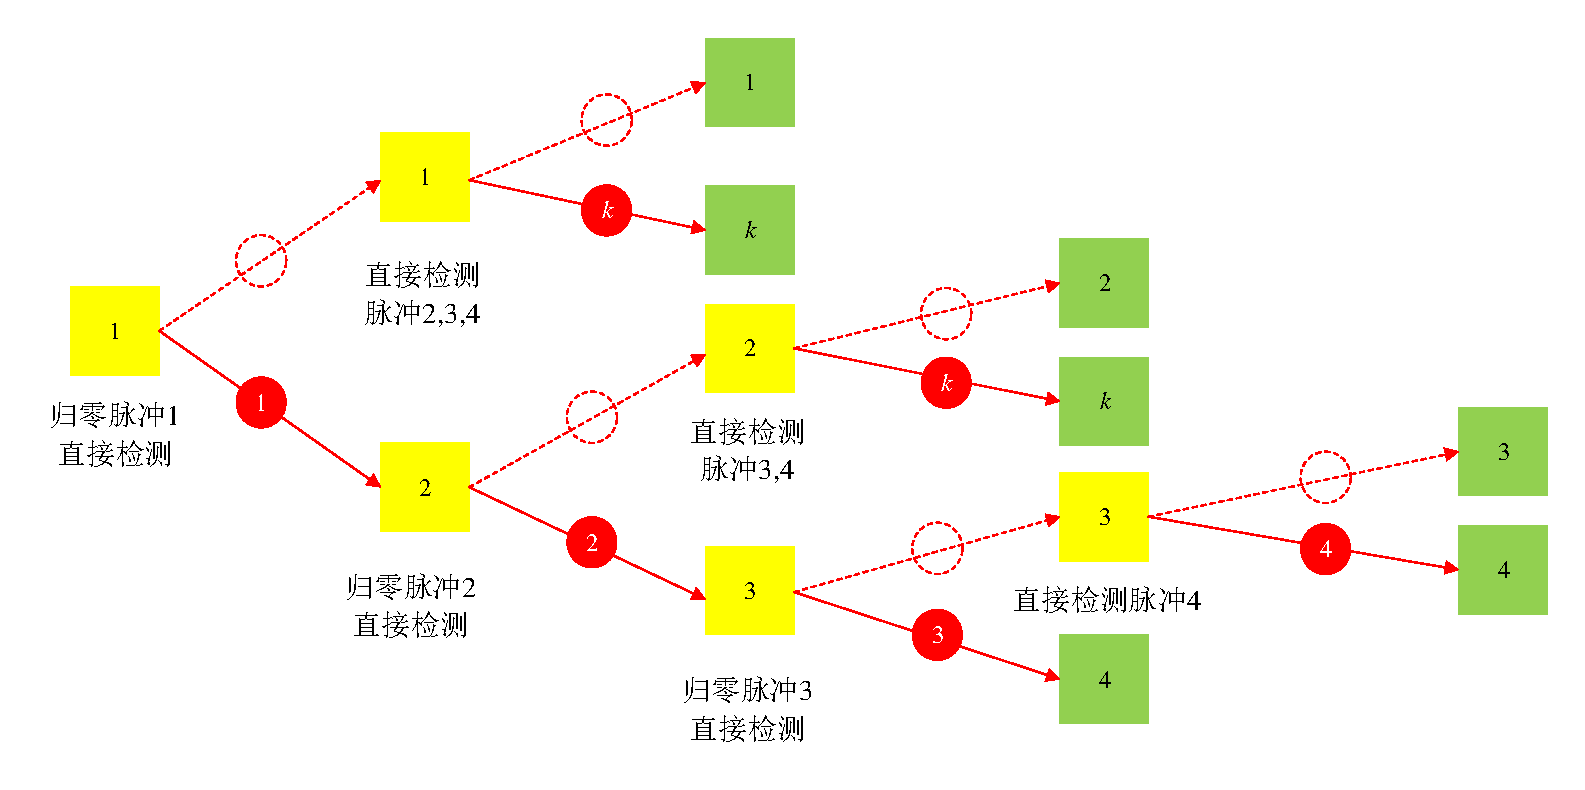
\includegraphics[width=\textwidth]{figures/chap2/CPN-Decision-Tree}
  \caption{4-PPM信号条件归零接收机反馈控制策略决策树}
  \label{fig:CPN-Decision-Tree}
\end{figure}

容易求得,条件归零接收机的平均错误概率为\cite{guha2011approaching,dolinar1982near}
\begin{equation}
P_e = \frac{1}{M}[(1-e^{-|\alpha|^2})^M + M e^{-|\alpha|^2} - 1].
\end{equation}
当光子数很大的时候,其渐近性能为
\begin{equation}
P_e \approx \frac{M-1}{2} e^{-2|\alpha|^2}.
\end{equation}
与式\ref{eq:PPM-Hel-error}对比,可以看到条件归零接收机与最优检测
在大光子数时只相差3dB。

与最优位移接收机思想类似,如果在条件归零接收机每一个时隙里,
采用不精确归零,则可进一步提升接收机在小信号时的性能\cite{guha2011approaching}。
2012年,这两种条件归零接收机被实验验证\cite{chen2012optical}。
Guha等人还提出,可以增加一个相敏放大器(PSA),
从而在位移操作上增加一个压缩操作,可以进一步提升
接收机的性能\cite{guha2011approaching}。
2014年,P. Dalla等人将条件归零接收机的控制策略
进一步改进,在每一个时隙里面采用Dolinar接收机
或者不精确归零接收机,并且每一个时隙的控制参数
都不相同,这些参数通过动态规划算法进行优化,
最终将接收机的性能进一步降低到非常接近Helstrom极限\cite{dalla2014adaptive}。



\subsection{其它类型量子接收机}
在上一小节,我们介绍了目前已经研究得比较多的
几种量子接收机实现方案。
除此之外,还有一些方案也值得借鉴和研究。
2013年,S. Guha等人提出针对任意相干态检测的量子接收机\cite{da2013achieving},
随后该研究组继续提出一种更方便实现的贯序波形归零(SWN)接收机,
用于实现任意相干态接收\cite{nair2014realizable}。
另外,K. Blume等人提出一种基于有限资源量子计算的量子接收机\cite{blume2012ideal},
为研究量子接收机提供新的思路。

与最小错误概率准则不同的是,基于最大无歧义概率准则设计的
无歧义态区分(USD)接收机也被研究人员关注,这种测量方案
理论上不存在错判的概率,但是存在无法判断的概率\cite{becerra2013implementation}。



\section{量子信道编码理论}

在经典信息论中,用Shannon熵来度量一个经典概率分布的不确定度\cite{jd2001xxlybm},
在量子信息论中,描述系统不确定度的是von Neumann熵,定义为\cite{nielsen2005qcqi,nielsen2010quantum}
\begin{equation}
S(\hat{\rho}) = -\Tr\left( \hat{\rho} \log_2 \hat{\rho} \right).
\end{equation}
$\hat{\rho}$是密度矩阵,若$\hat{\rho}$的特征值为$\lambda_x$,
那么上式可以改写为
\begin{equation}
S(\hat{\rho}) = -\sum_x \lambda_x \log_2 \lambda_x.
\end{equation}
这与Shannon熵的形式一致,
为方便记,可以定义$0\log_2 0=0$,便于后续表达。

通过量子信道传递经典信息
需要在发送端将要发送的符号$x \in X$
映射到对应的量子态$\hat{\rho}_x$,然后
将它发送出去,设该信道为$\mathcal{H}$,
每一个量子态对应的先验概率为$p_x$。
这些量子态构成一个混合量子态$\sum_x p_x\hat{\rho}_x$,它的熵满足如下不等式\cite{nielsen2005qcqi}
\begin{equation}
\sum_x p_x S(\hat{\rho}_x) \le S(\sum_x p_x\hat{\rho}_x) \le \sum_x p_x S(\hat{\rho}_x) + H(p_x).
\label{eq:QI-low-up-bound}
\end{equation}
其中$H(p_x)$表示先验分布$p_i$的Shannnon熵。

在接收端,接收机采用一组POVM测量$\hat{\Pi}_y$
进行探测,每一个测量对应的输出为$y \in Y$,
探测的条件概率为
\begin{equation}
P(x|y) = \Tr(\Pi_x \hat{\rho}_y ).
\end{equation}
那么该系统传递的交互信息量为
\begin{equation}
I_1(p_x, \hat{\Pi}_x) = \sum_x p_x \sum_y P(y|x) \log_2  \frac{P(y|x)}{\sum_z p_z P(y|z)}.
\end{equation}
对于给定的符号集合,记交互信息量的最大值为
\begin{equation}
C_1= \sup_{p_x,\hat{\Pi}_y} I_1(p_x, \hat{\Pi}_x).
\end{equation}
它是通过该符号集合对应的单个量子信道$\mathcal{H}$
所能获取的最大信息量。


与上述类似的讨论,我们考虑该单个量子信道的直积信道
$\mathcal{H}^{\otimes n}=\mathcal{H}\otimes\cdots \otimes \mathcal{H}$,
此时输入符号集合为$X^n$,对于其中的每一个符号序列$u = (x_1, x_2, ..., x_n)$,
我们将它映射到直积态
\begin{equation}
\hat{\rho}_u = \hat{\rho}_{x_1}\otimes \hat{\rho}_{x_2}\otimes \cdots \otimes \hat{\rho}_{x_n}.
\end{equation}
设$p_u$是该序列的先验概率,接收端采用POVM测量$\hat{\Pi}_u$进行探测,
我们可以得到交互信息量$I_n(p_u, \hat{\rho}_u)$,
记交互信息量最大值为
\begin{equation}
C_n= \sup_{p_u,\hat{\Pi}_u} I_n(p_u, \hat{\Pi}_u).
\end{equation}
它满足超加性
\begin{equation}
C_n + C_m \le C_{n+m}
\end{equation}
在经典的无记忆信道中,只能取等号,
在量子信道中,可以取不等号,
它存在极限
\begin{equation}
C = \lim_{n \rightarrow \infty} C_n / n.
\end{equation}
该极限被称为信道$\mathcal{H}$的信道容量。
经过A. S. Holevo, P. Hausladen,W. K. Wootters等人的努力,
证明了对任意量子态$\{\hat{\rho}_x\}$,信道$\mathcal{H}$的容量为\cite{holevo1973bounds,hausladen1996classical, holevo1996capacity}
\begin{equation}
C = \max_{p_x}\left[ S(\sum_x p_x \hat{\rho}_x) - \sum_x p_x S( \hat{\rho}_x) \right].
\end{equation}
这个容量也称为量子信道$\mathcal{H}$的Holevo容量。
利用式\ref{eq:QI-low-up-bound},可知
\begin{equation}
C \le \max_{p_x}H(p_x).
\end{equation}
当且仅当各量子态之间互相正交时取等号。

如果将量子态放宽到任意量子态,
可以证明,对于能量和带宽受限的条件下,
玻色子场可以最大化信道容量\cite{yuen1993ultimate}。
取符号集合$X = \mathbb{N}$,
$\hat{\rho}_n = \ket{n}\bra{n}$为Fork态,
且先验分布$p_n= N^n(1+N)^{-(n+1)}$,
其中$N$为发送的平均光子数。
此时具有的最大容量
\begin{equation}
C(N) = (N+1)\log_2(N+1) -N \log_2 N.
\label{eq:Boson-capacity}
\end{equation}


量子信道编码定理指出,可以通过对某些特定的长度为$N$的编码码字,
进行联合检测,就有可能随着长度$N$的增大,交互信息量
可以任意逼近Holevo容量\cite{hausladen1996classical, holevo1996capacity}。
因此,两个重要的任务就是找到合适的编码以及
有效的联合检测方案。
1996年,Hausladen采用随机编码和平方根检测的方案
证实对纯态信号集合可以逼近Holevo容量。
近年来,结构化光学接收机\cite{guha2011structured}、
序贯测量方案\cite{giovannetti2012achieving}
以及无歧义态区分方案\cite{takeoka2013achieving}
逼近Holevo容量已被报道。
此外通过极化编码和平方根检测的方案也
被证明可以逼近Holevo容量\cite{guha2012polar}。
但是这些接收机实现都还比较复杂,
不利于工程实现,因此探索方便工程实现的
联合检测接收机是一件十分重要的事情。



